\documentclass[12pt]{article}
\usepackage{times} 			% use Times New Roman font

\usepackage[margin=1in]{geometry}   % sets 1 inch margins on all sides
\usepackage{hyperref}               % for URL formatting
\usepackage[pdftex]{graphicx}       % So includegraphics will work
\setlength{\parskip}{1em}           % skip 1em between paragraphs
\usepackage{indentfirst}            % indent the first line of each paragraph
\usepackage{datetime}
\usepackage[small, bf]{caption}
\usepackage{listings}               % for code listings
\usepackage{xcolor}                 % for styling code
\usepackage{multirow}

%New colors defined below
\definecolor{backcolour}{RGB}{246, 246, 246}   % 0xF6, 0xF6, 0xF6
\definecolor{codegreen}{RGB}{16, 124, 2}       % 0x10, 0x7C, 0x02
\definecolor{codepurple}{RGB}{170, 0, 217}     % 0xAA, 0x00, 0xD9
\definecolor{codered}{RGB}{154, 0, 18}         % 0x9A, 0x00, 0x12

%Code listing style named "gcolabstyle" - matches Google Colab
\lstdefinestyle{gcolabstyle}{
  basicstyle=\ttfamily\small,
  backgroundcolor=\color{backcolour},   
  commentstyle=\itshape\color{codegreen},
  keywordstyle=\color{codepurple},
  stringstyle=\color{codered},
  numberstyle=\ttfamily\footnotesize\color{darkgray}, 
  breakatwhitespace=false,         
  breaklines=true,                 
  captionpos=b,                    
  keepspaces=true,                 
  numbers=left,                    
  numbersep=5pt,                  
  showspaces=false,                
  showstringspaces=false,
  showtabs=false,                  
  tabsize=2
}

\lstset{style=gcolabstyle}      %set gcolabstyle code listing

% to make long URIs break nicely
\makeatletter
\g@addto@macro{\UrlBreaks}{\UrlOrds}
\makeatother

% for fancy page headings
\usepackage{fancyhdr}
\setlength{\headheight}{13.6pt} % to remove fancyhdr warning
\pagestyle{fancy}
\fancyhf{}
\rhead{\small \thepage}
\lhead{\small HW 4\, Venkatesh}  % EDIT THIS, REPLACE # with HW number
\chead{\small CS 532, Fall 2021} 

%-------------------------------------------------------------------------
\begin{document}

% EDIT THE ITEMS HERE
\begin{centering}
{\large\textbf{HW 4\ - Exploring Social Networks}}\\ 
Swathi Venkatesh\\
11/02/2021\\
\end{centering}

%-------------------------------------------------------------------------

% The * after \section just says to not number the sections
\section*{Q1}
Determine if the friendship paradox holds for a user's Facebook account. (This used to be more interesting when you could more easily download your friend's friends data from Facebook. Facebook now requires each friend to approve this operation, effectively making it impossible.)

HW4-friend-count.csv contains a user's friends' names and number of friends they each have. (You'll need to accept the GitHub Classroom invite to get this datafile.)

\emph{Q: What is the mean, standard deviation, and median of the number of friends that the user's friends have?}

\subsection*{Answer}

%Python code highlighting
\begin{lstlisting}[language=Python, caption=frienshipParadox.py , label=lst:copy]
#!/usr/local/bin/python3
import matplotlib.pyplot as plt
import pandas as pd
f = "HW4-friend-count.csv"
df = pd.read_csv(f,index_col=False, encoding='utf-8')
#remove extra spaces from columns
df.columns =[col.strip() for col in df.columns]
df = df.sort_values(by="FRIENDCOUNT")

#create a list of new users
newuser= []
for x  in range(98):
    c =  str(x)
    newuser.append(c)
# replace this new list to the column user in the df
df.USER = newuser
print('The mean is',df.FRIENDCOUNT.mean())
print('The std deviation is',df.FRIENDCOUNT.std())
print('The median is',df.FRIENDCOUNT.median())
#plot the values
plt.rcParams['figure.figsize'] =20,40
plt.rcParams['font.size'] = 12;
plt.plot(df.USER,df.FRIENDCOUNT,marker='o')
plt.grid(True)
plt.xlabel(xlabel = "friends", fontsize=20)
plt.ylabel(ylabel= "no. of friends", fontsize=20)
plt.legend(loc=6,fontsize=25);
plt.gca().invert_xaxis()
plt.show()


\end{lstlisting}



\begin{figure}[h]
    \centering
    % trim and clip are used to crop the image, trim=left bottom right top
    % width sets max width, height will be scaled appropriately
    
\includegraphics[trim=0 0 0 8, clip, width=\textwidth] {Capture1.PNG}
    \caption{Mean, standard deviation and median}
    \label{fig:web-growth}
\end{figure}

\begin{figure}[h]
    \centering
    % trim and clip are used to crop the image, trim=left bottom right top
    % width sets max width, height will be scaled appropriately
    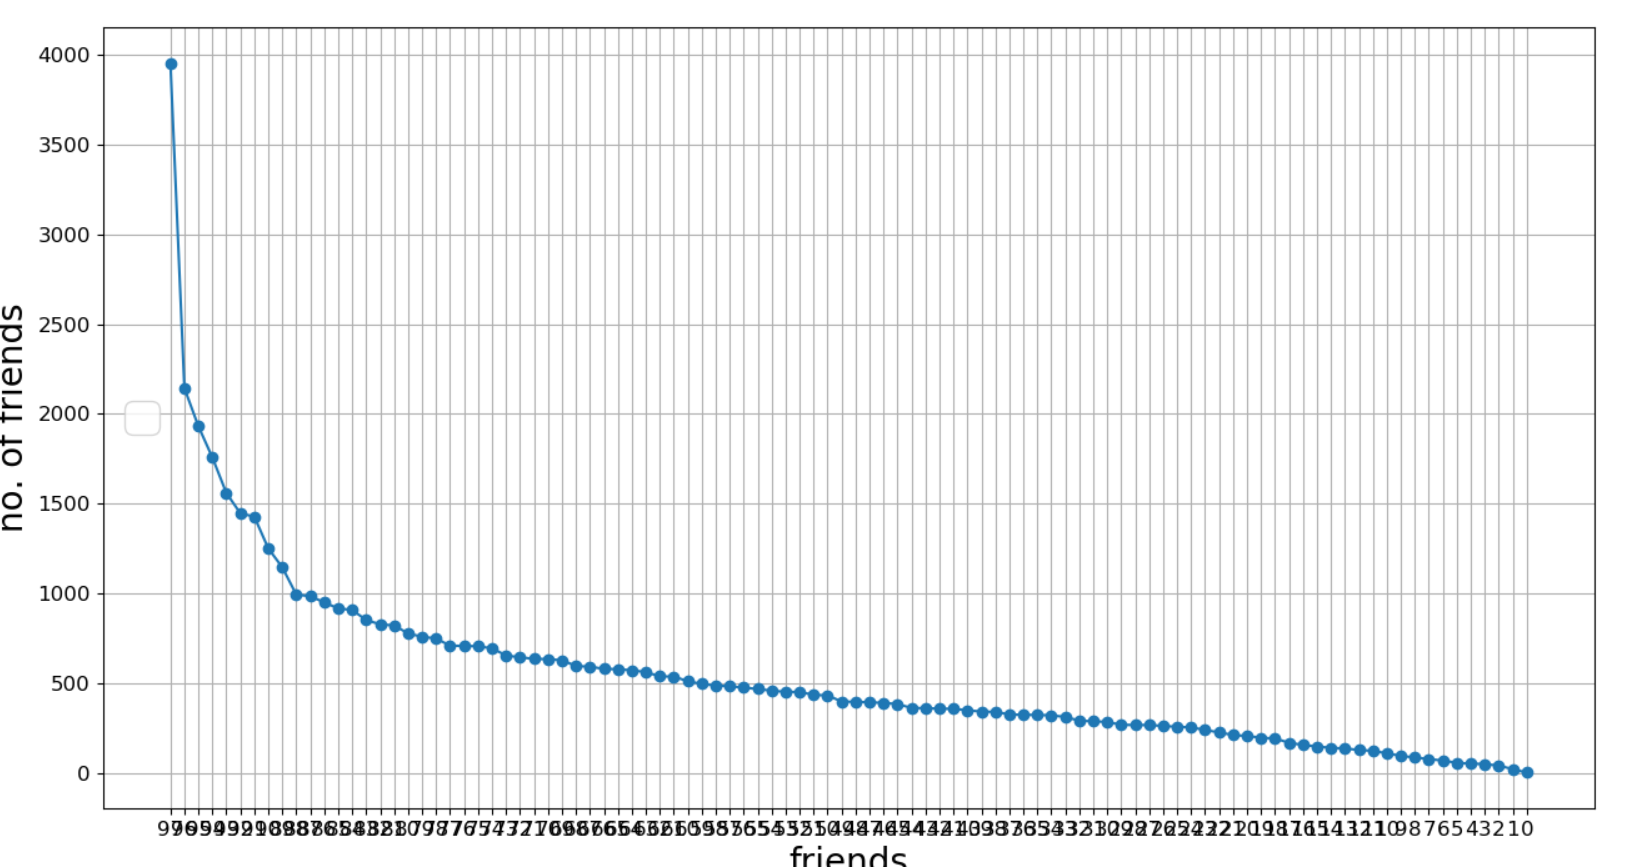
\includegraphics[trim=0 0 0 8, clip, width=\textwidth] {Capture.PNG}
    \caption{Plot for Q1}
    \label{fig:web-growth}
\end{figure}

\emph{Q: Does the friendship paradox hold for this user and their friends on Facebook?}

\emph{Ans:} Yes, friendship paradox hold for this user and their friends on Facebook.

\subsection*{Discussion}

I read the csv file using the pandas library. Then, sorted the values of the FriendCount column. 

I replaced the user column in dataframe with list values. Using the built dataframe I calculated the mean, standard deviation and median. Finally plotted the graph as shown in Figure 2. As, the friend with the most friends should be on the left side of the graph I used plt.gca().invert\_xaxis() for the same.

The mean is 542.6734693877551

The std deviation is 539.4337385239659

The median is 396.0




\section*{Q2}
Determine if the friendship paradox holds for your Twitter account. Since Twitter is a directed graph, use followers as the value you measure (i.e., "do your followers have more followers than you?").

If you have less than 50 followers on Twitter, then you can do the analysis for another Twitter account (e.g., my account is weiglemc) and substitute the user you pick for you in the questions below.

\emph{Q: What is the mean, standard deviation, and median of the number of followers that your followers have?}







\subsection*{Answer}
%Python code highlighting
\begin{lstlisting}[language=Python, caption=twitterFoll.py , label=lst:copy]
#!/usr/local/bin/python3
#import necessary libraries
import pandas as pd
from twarc.client2 import Twarc2
import matplotlib.pyplot as plt
import itertools

def auth():#authorization 
    bearer_token="AAAAAAAAAAAAAAAAAAAAAJ2AUAEAAAAALRZWrij70cG9YMLEBV1l2uq7aPY%3Ddacuw3kcsTgmfyCnftWr8tM98XNOGof3lnxuXCh6W9c6Rlp0CJ"
    tw = Twarc2(bearer_token=bearer_token)
    return tw
def plot_data(df,fwfing):
    plt.rcParams['figure.figsize'] =40,25
    plt.rcParams['font.size'] = 17;
    plt.plot(df.USER,df.FRIENDCOUNT, label="FriendCount",marker='o')
    plt.grid(True)
    plt.xticks(rotation=90)
    plt.xlabel(xlabel = "friends", fontsize=20)
    plt.ylabel(ylabel= "no. of friends", fontsize=20)
    plt.legend(loc=6,fontsize=25);
    plt.gca().invert_xaxis()
    return plt.show()
def df_replacement(df):
    df = df.sort_values(by="FRIENDCOUNT")
    #create a list of new users
    newUser= []
    try:
        for x  in range(len(df)):
            c = str(x)
            newUser.append(c)
        # replace this new list to the column user in the dataframe
        df.USER = newUser
    except Exception as p:
        print(p)
    return df
def get_number_of_followers(id,i):
    #get user 
    user = auth().followers(id)
    try:
        if i == 0:
            fwers_flowing = user.followers_count
    except Exception as p:
        print(p)
    return user.screen_name,fwers_flowing
def getUserFollowers(screen_name):
   users = []
   followersC = []
    #followers
   
   p= auth().user_lookup(users=n,usernames=True)
   c =1
   for ps in p:
       #parse in 0 to get the followers count
       us, count = get_number_of_followers(ps,0)
       users.append(us)
       followersC.append(count)
       c=c +1
       if(c > 179):
           break;
   
   prod = pd.DataFrame(list(zip(users,followersC)))
   prod.columns = ["USER", "FRIENDCOUNT"]
   #sort and replace the names symbol fn
   prod = df_replacement(prod)
   return prod
screen_name = "iAchieveODU"
try:
   
   f = getUserFollowers(screen_name)
   #print the mean, std and median
   print("The mean is {}".format(f.FRIENDCOUNT.mean()))
   print("The std deviation is {}".format(f.FRIENDCOUNT.std()))
   print("The median is {}".format(f.FRIENDCOUNT.median()))
   #print as a csv file
   f.to_csv("followers.csv",index=False)
   #plot the graph
   plot_data(f,0)
\end{lstlisting}

\begin{figure}[h]
    \centering
    % trim and clip are used to crop the image, trim=left bottom right top
    % width sets max width, height will be scaled appropriately
    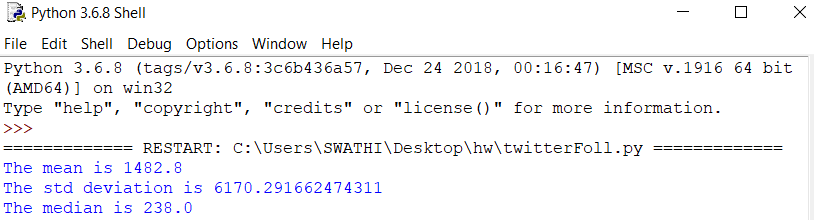
\includegraphics[trim=0 0 0 0, clip, width=\textwidth] {Capture3.PNG}
    \caption{Mean, standard deviation and median}
    \label{fig:web-growth}
\end{figure}

\begin{figure}[h]
    \centering
    % trim and clip are used to crop the image, trim=left bottom right top
    % width sets max width, height will be scaled appropriately
    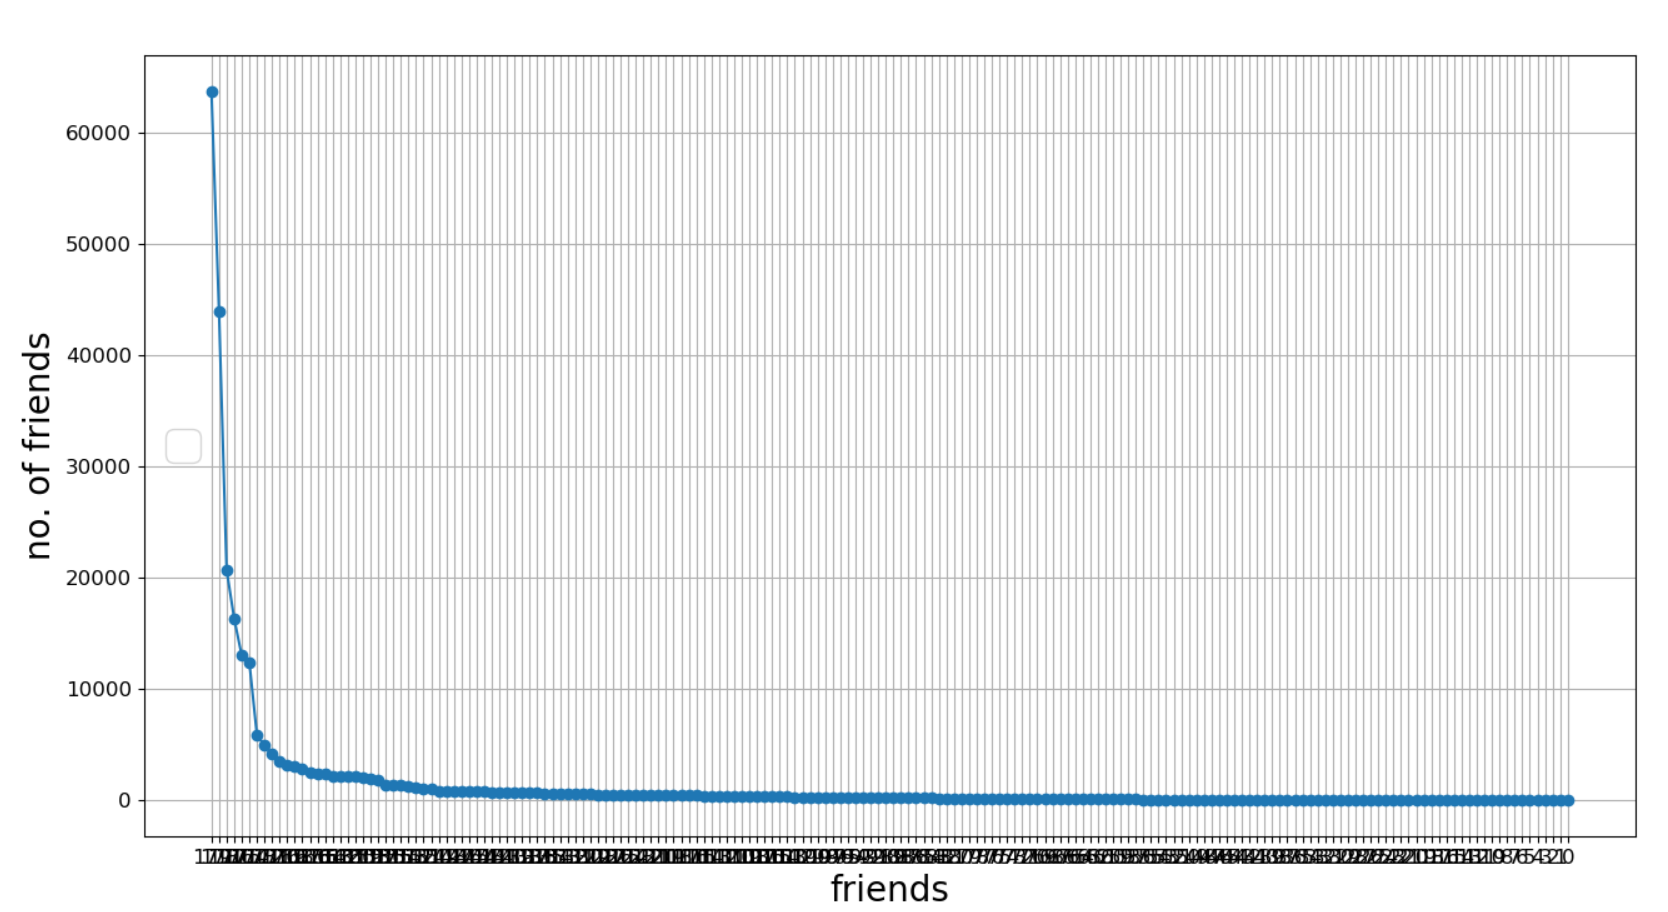
\includegraphics[trim=0 0 0 8, clip, width=\textwidth] {Capture2.PNG}
    \caption{Plot for Q2}
    \label{fig:web-growth}
\end{figure}
\subsection*{Discussion}
I created a function getUserFollowers and used the screen name iAchieveODU and retrieved all followers id.

I passed the user id to get\_number\_of\_followers and this returns the followers count of the associated user id. 

I parsed the generated list of users and followers count as pandas dataframe to df\_replacement and performed similar operation as Q1 and got the dataframe and found the values of the mean, standard deviation and median.

The mean is 1482.8

The std deviation is 6170.291662474311

The median is 238.0

And then plotted the graph as shown in Figure 4.


\emph{Q: Does the friendship paradox hold for you and your followers on Twitter?}

\emph{Ans.} Comparing the mean of iAchieveODU's  followers followers count 1482.8 to  iAchieveODU's  followers  count of 176. Those that they follow have a higher followers count than iAChieveODU has.

\section*{References}
\begin{itemize}
    \item {Twitter, \url{https://scholarslab.github.io/learn-twarc/06-twarc-command-basics}}
    \item {Github , \url{https://github.com/DocNow/twarc}}
    \item {Twitter data , \url{https://twittercommunity.com/t/downloading-friends-from-a-list-of-users/155024}}
    \item {Matplotlib,
    \url{https://matplotlib.org/3.2.2/gallery/misc/plotfile_demo_sgskip.html}}
   \item {Matplotlib Subplots,
    \url{https://matplotlib.org/stable/gallery/subplots_axes_and_figures/invert_axes.html}}
   
    
\end{itemize} 

\end{document}
\end{document}
